% Options for packages loaded elsewhere
\PassOptionsToPackage{unicode}{hyperref}
\PassOptionsToPackage{hyphens}{url}
%
\documentclass[
]{article}
\usepackage{amsmath,amssymb}
\usepackage{lmodern}
\usepackage{ifxetex,ifluatex}
\ifnum 0\ifxetex 1\fi\ifluatex 1\fi=0 % if pdftex
  \usepackage[T1]{fontenc}
  \usepackage[utf8]{inputenc}
  \usepackage{textcomp} % provide euro and other symbols
\else % if luatex or xetex
  \usepackage{unicode-math}
  \defaultfontfeatures{Scale=MatchLowercase}
  \defaultfontfeatures[\rmfamily]{Ligatures=TeX,Scale=1}
\fi
% Use upquote if available, for straight quotes in verbatim environments
\IfFileExists{upquote.sty}{\usepackage{upquote}}{}
\IfFileExists{microtype.sty}{% use microtype if available
  \usepackage[]{microtype}
  \UseMicrotypeSet[protrusion]{basicmath} % disable protrusion for tt fonts
}{}
\makeatletter
\@ifundefined{KOMAClassName}{% if non-KOMA class
  \IfFileExists{parskip.sty}{%
    \usepackage{parskip}
  }{% else
    \setlength{\parindent}{0pt}
    \setlength{\parskip}{6pt plus 2pt minus 1pt}}
}{% if KOMA class
  \KOMAoptions{parskip=half}}
\makeatother
\usepackage{xcolor}
\IfFileExists{xurl.sty}{\usepackage{xurl}}{} % add URL line breaks if available
\IfFileExists{bookmark.sty}{\usepackage{bookmark}}{\usepackage{hyperref}}
\hypersetup{
  pdftitle={USDA National School Lunch Program Time Series Analysis},
  pdfauthor={Scout Leonard},
  hidelinks,
  pdfcreator={LaTeX via pandoc}}
\urlstyle{same} % disable monospaced font for URLs
\usepackage[margin=1in]{geometry}
\usepackage{color}
\usepackage{fancyvrb}
\newcommand{\VerbBar}{|}
\newcommand{\VERB}{\Verb[commandchars=\\\{\}]}
\DefineVerbatimEnvironment{Highlighting}{Verbatim}{commandchars=\\\{\}}
% Add ',fontsize=\small' for more characters per line
\usepackage{framed}
\definecolor{shadecolor}{RGB}{248,248,248}
\newenvironment{Shaded}{\begin{snugshade}}{\end{snugshade}}
\newcommand{\AlertTok}[1]{\textcolor[rgb]{0.94,0.16,0.16}{#1}}
\newcommand{\AnnotationTok}[1]{\textcolor[rgb]{0.56,0.35,0.01}{\textbf{\textit{#1}}}}
\newcommand{\AttributeTok}[1]{\textcolor[rgb]{0.77,0.63,0.00}{#1}}
\newcommand{\BaseNTok}[1]{\textcolor[rgb]{0.00,0.00,0.81}{#1}}
\newcommand{\BuiltInTok}[1]{#1}
\newcommand{\CharTok}[1]{\textcolor[rgb]{0.31,0.60,0.02}{#1}}
\newcommand{\CommentTok}[1]{\textcolor[rgb]{0.56,0.35,0.01}{\textit{#1}}}
\newcommand{\CommentVarTok}[1]{\textcolor[rgb]{0.56,0.35,0.01}{\textbf{\textit{#1}}}}
\newcommand{\ConstantTok}[1]{\textcolor[rgb]{0.00,0.00,0.00}{#1}}
\newcommand{\ControlFlowTok}[1]{\textcolor[rgb]{0.13,0.29,0.53}{\textbf{#1}}}
\newcommand{\DataTypeTok}[1]{\textcolor[rgb]{0.13,0.29,0.53}{#1}}
\newcommand{\DecValTok}[1]{\textcolor[rgb]{0.00,0.00,0.81}{#1}}
\newcommand{\DocumentationTok}[1]{\textcolor[rgb]{0.56,0.35,0.01}{\textbf{\textit{#1}}}}
\newcommand{\ErrorTok}[1]{\textcolor[rgb]{0.64,0.00,0.00}{\textbf{#1}}}
\newcommand{\ExtensionTok}[1]{#1}
\newcommand{\FloatTok}[1]{\textcolor[rgb]{0.00,0.00,0.81}{#1}}
\newcommand{\FunctionTok}[1]{\textcolor[rgb]{0.00,0.00,0.00}{#1}}
\newcommand{\ImportTok}[1]{#1}
\newcommand{\InformationTok}[1]{\textcolor[rgb]{0.56,0.35,0.01}{\textbf{\textit{#1}}}}
\newcommand{\KeywordTok}[1]{\textcolor[rgb]{0.13,0.29,0.53}{\textbf{#1}}}
\newcommand{\NormalTok}[1]{#1}
\newcommand{\OperatorTok}[1]{\textcolor[rgb]{0.81,0.36,0.00}{\textbf{#1}}}
\newcommand{\OtherTok}[1]{\textcolor[rgb]{0.56,0.35,0.01}{#1}}
\newcommand{\PreprocessorTok}[1]{\textcolor[rgb]{0.56,0.35,0.01}{\textit{#1}}}
\newcommand{\RegionMarkerTok}[1]{#1}
\newcommand{\SpecialCharTok}[1]{\textcolor[rgb]{0.00,0.00,0.00}{#1}}
\newcommand{\SpecialStringTok}[1]{\textcolor[rgb]{0.31,0.60,0.02}{#1}}
\newcommand{\StringTok}[1]{\textcolor[rgb]{0.31,0.60,0.02}{#1}}
\newcommand{\VariableTok}[1]{\textcolor[rgb]{0.00,0.00,0.00}{#1}}
\newcommand{\VerbatimStringTok}[1]{\textcolor[rgb]{0.31,0.60,0.02}{#1}}
\newcommand{\WarningTok}[1]{\textcolor[rgb]{0.56,0.35,0.01}{\textbf{\textit{#1}}}}
\usepackage{graphicx}
\makeatletter
\def\maxwidth{\ifdim\Gin@nat@width>\linewidth\linewidth\else\Gin@nat@width\fi}
\def\maxheight{\ifdim\Gin@nat@height>\textheight\textheight\else\Gin@nat@height\fi}
\makeatother
% Scale images if necessary, so that they will not overflow the page
% margins by default, and it is still possible to overwrite the defaults
% using explicit options in \includegraphics[width, height, ...]{}
\setkeys{Gin}{width=\maxwidth,height=\maxheight,keepaspectratio}
% Set default figure placement to htbp
\makeatletter
\def\fps@figure{htbp}
\makeatother
\setlength{\emergencystretch}{3em} % prevent overfull lines
\providecommand{\tightlist}{%
  \setlength{\itemsep}{0pt}\setlength{\parskip}{0pt}}
\setcounter{secnumdepth}{-\maxdimen} % remove section numbering
\ifluatex
  \usepackage{selnolig}  % disable illegal ligatures
\fi

\title{USDA National School Lunch Program Time Series Analysis}
\author{Scout Leonard}
\date{11/16/2021}

\begin{document}
\maketitle

\begin{Shaded}
\begin{Highlighting}[]
\FunctionTok{library}\NormalTok{(here)}
\FunctionTok{library}\NormalTok{(lubridate)}
\FunctionTok{library}\NormalTok{(tidyverse)}
\FunctionTok{library}\NormalTok{(zoo)}
\FunctionTok{library}\NormalTok{(feasts)}
\FunctionTok{library}\NormalTok{(tsibble)}
\FunctionTok{library}\NormalTok{(patchwork)}
\FunctionTok{library}\NormalTok{(grid)}
\FunctionTok{library}\NormalTok{(ggplotify)}

\FunctionTok{options}\NormalTok{(}\AttributeTok{scipen =} \DecValTok{999}\NormalTok{)}
\end{Highlighting}
\end{Shaded}

\hypertarget{my-question}{%
\section{My Question:}\label{my-question}}

My analysis seeks to explore the questions: Is there seasonality in how
U.S. school food programs feed students? What about long-term trends,
and how did any trends change in 2020 during school closures from the
Covid-19 pandemic?

\hypertarget{background}{%
\subsection{Background}\label{background}}

The National School Lunch Program (NSLP) is an enormous food system with
major implications for equity in American K-12 education systems. Every
day, NSLP provides \textasciitilde30 million children school lunch at
free or reduced prices (1). It operates in public and nonprofit private
schools and residential childcare facilities (2).

To provide meals at free and reduced cost to students, participating
school districts are reimbursed cash subsidies for every qualifying meal
they serve. To qualify for subsidy, meals served by Nutrition Services
operators must meet federal meal pattern policies which define meal
content around qualifying food group combinations, sugar content, etc.

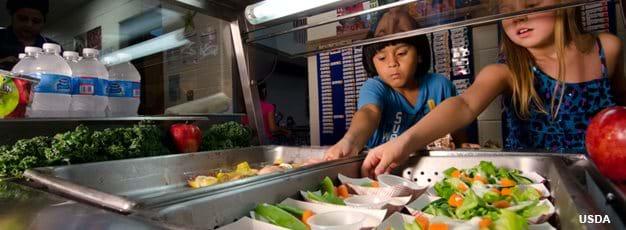
\includegraphics{lunch_image.jpg}

**** something about impact of access to nutrition on student behavior
and performace, with sources cited!

\hypertarget{data-description}{%
\section{Data Description}\label{data-description}}

The Food and Nutrition Services sector of the USDA offers
\href{https://www.fns.usda.gov/data-research}{monthly and annual
reports} of national participation in the National School Lunch Program
and other school meal programs subsidized by the USDA (breakfast,
seamless summer, supper, and snacks).

To answer my questions\ldots{}

\textbf{My analysis seeks to explore the questions: Is there seasonality
in how U.S. school food programs feed students? What about long-term
trends, and how did any trends change in 2020 during school closures
from the Covid-19 pandemic? }

\ldots{} I used the National Level Monthly Data for the National School
Lunch Program, which comes in PDF and Excel formats which are public. I
downloaded the Excel format of the monthly data and did some tidying in
Excel to make sure the .csv version would be friendly with R! There were
some formatting thing like merged cells that included titles, not
observations, as rows, which I eliminated before downloading as a .csv
in my R project.

\begin{Shaded}
\begin{Highlighting}[]
\CommentTok{\#read in the monthly lunch data }
\NormalTok{usda\_monthly }\OtherTok{\textless{}{-}} \FunctionTok{read.csv}\NormalTok{(}\FunctionTok{here}\NormalTok{(}\StringTok{"data"}\NormalTok{, }\StringTok{"usda\_monthly\_data\_tidy.csv"}\NormalTok{))}
\end{Highlighting}
\end{Shaded}

Even after a little manipulation in excel, there were changes to be made
for easier manipulation of my monthly lunch data dataframe. Here, I give
columns more descriptive names, remove odd columns that were added to
the dataframe when I read in the .csv, mutate columns to exclude ``\%''
``-'' or spaces that R cannot make sense of.

\begin{Shaded}
\begin{Highlighting}[]
\CommentTok{\#change first column name }
\FunctionTok{colnames}\NormalTok{(usda\_monthly)[}\DecValTok{1}\NormalTok{] }\OtherTok{\textless{}{-}} \StringTok{"month"}

\CommentTok{\#delete the weird columns that got added between downloading the raw data to my }
\CommentTok{\#local computer and reading it to .Rmd}
\NormalTok{usda\_monthly }\OtherTok{\textless{}{-}} \FunctionTok{select}\NormalTok{(usda\_monthly, }\SpecialCharTok{{-}}\FunctionTok{c}\NormalTok{(}\StringTok{"X"}\NormalTok{, }\StringTok{"X.1"}\NormalTok{))}

\CommentTok{\#change last column name}
\FunctionTok{colnames}\NormalTok{(usda\_monthly)[}\DecValTok{9}\NormalTok{] }\OtherTok{\textless{}{-}} \StringTok{"fiscal\_year"}
\end{Highlighting}
\end{Shaded}

\begin{Shaded}
\begin{Highlighting}[]
\CommentTok{\#remove percent signs from percent\_free\_of\_total\_lunches and }
\CommentTok{\#percent\_reduced\_price\_of\_total\_lunches columns}
\NormalTok{usda\_monthly }\OtherTok{\textless{}{-}}\NormalTok{ usda\_monthly }\SpecialCharTok{\%\textgreater{}\%} 
 \FunctionTok{mutate}\NormalTok{(}\AttributeTok{percent\_free\_of\_total\_lunches =} \FunctionTok{gsub}\NormalTok{(}\StringTok{\textquotesingle{}\%\textquotesingle{}}\NormalTok{,}\StringTok{\textquotesingle{}\textquotesingle{}}\NormalTok{, percent\_free\_of\_total\_lunches)) }\SpecialCharTok{\%\textgreater{}\%} 
  \FunctionTok{mutate}\NormalTok{(}\AttributeTok{percent\_reduced\_price\_of\_total\_lunches =} \FunctionTok{gsub}\NormalTok{(}\StringTok{\textquotesingle{}\%\textquotesingle{}}\NormalTok{,}\StringTok{\textquotesingle{}\textquotesingle{}}\NormalTok{,percent\_reduced\_price\_of\_total\_lunches)) }\SpecialCharTok{\%\textgreater{}\%}
  \FunctionTok{mutate}\NormalTok{(}\AttributeTok{month =} \FunctionTok{gsub}\NormalTok{(}\StringTok{"{-}"}\NormalTok{, }\StringTok{" "}\NormalTok{, month))}
\end{Highlighting}
\end{Shaded}

Last, I make sure the class of each column is correct. All of the
columns were of class \texttt{numeric} when read in, so I mutated the
\texttt{month} column to \texttt{yearmon} using the \texttt{zoo}
package, and everything else to numeric.

\begin{Shaded}
\begin{Highlighting}[]
\CommentTok{\#convert month column to class datetime from class character}
\NormalTok{usda\_monthly }\OtherTok{\textless{}{-}}\NormalTok{ usda\_monthly }\SpecialCharTok{\%\textgreater{}\%} 
  \FunctionTok{mutate}\NormalTok{(}\StringTok{"month"} \OtherTok{=}\NormalTok{ zoo}\SpecialCharTok{::}\FunctionTok{as.yearmon}\NormalTok{(month, }\StringTok{"\%y \%b"}\NormalTok{))}

\CommentTok{\#check class of all columns}
\FunctionTok{lapply}\NormalTok{(usda\_monthly, class)}

\CommentTok{\#the data in most of the columns is of class character, but needs to be numeric}
\NormalTok{usda\_monthly }\OtherTok{\textless{}{-}}\NormalTok{ usda\_monthly }\SpecialCharTok{\%\textgreater{}\%} 
  \FunctionTok{mutate\_if}\NormalTok{(is.character, as.numeric)}
\end{Highlighting}
\end{Shaded}

Finally, to have an initial look at my data, I make simple line graphs
here:

\begin{Shaded}
\begin{Highlighting}[]
\CommentTok{\#total lunches served plot }
\NormalTok{total\_lunches\_testplot }\OtherTok{\textless{}{-}} \FunctionTok{ggplot}\NormalTok{(}\AttributeTok{data =}\NormalTok{ usda\_monthly, }\FunctionTok{aes}\NormalTok{(}\AttributeTok{x =}\NormalTok{ month, }\AttributeTok{y =}\NormalTok{ total\_lunches\_served)) }\SpecialCharTok{+}
  \FunctionTok{geom\_line}\NormalTok{(}\AttributeTok{color =} \StringTok{"darkcyan"}\NormalTok{) }\SpecialCharTok{+}
  \FunctionTok{theme\_minimal}\NormalTok{() }\SpecialCharTok{+}
  \FunctionTok{labs}\NormalTok{(}\AttributeTok{title =} \StringTok{"NSLP Lunches Served (Monthly)"}\NormalTok{,}
       \AttributeTok{x =} \StringTok{"Month"}\NormalTok{,}
       \AttributeTok{y =} \StringTok{"Total Lunches Served"}\NormalTok{)}

\NormalTok{usda\_monthly }\OtherTok{\textless{}{-}}\NormalTok{ usda\_monthly }\SpecialCharTok{\%\textgreater{}\%} 
  \FunctionTok{mutate}\NormalTok{(}\AttributeTok{total\_free\_lunches =}\NormalTok{ total\_lunches\_served }\SpecialCharTok{*}\NormalTok{ percent\_free\_of\_total\_lunches)}

\NormalTok{monthly\_free\_testplot }\OtherTok{\textless{}{-}} \FunctionTok{ggplot}\NormalTok{(}\AttributeTok{data =}\NormalTok{ usda\_monthly, }\FunctionTok{aes}\NormalTok{(}\AttributeTok{x =}\NormalTok{ month, }\AttributeTok{y =}\NormalTok{ total\_free\_lunches)) }\SpecialCharTok{+}
  \FunctionTok{geom\_line}\NormalTok{(}\AttributeTok{color =} \StringTok{"darkcyan"}\NormalTok{) }\SpecialCharTok{+}
  \FunctionTok{theme\_minimal}\NormalTok{() }\SpecialCharTok{+}
  \FunctionTok{labs}\NormalTok{(}\AttributeTok{title =} \StringTok{"NSLP Free Lunches Served (Monthly)"}\NormalTok{,}
       \AttributeTok{x =} \StringTok{"Month"}\NormalTok{,}
       \AttributeTok{y =} \StringTok{"Total Lunches Served"}\NormalTok{)}

\NormalTok{total\_lunches\_testplot }\SpecialCharTok{/}\NormalTok{ monthly\_free\_testplot}
\end{Highlighting}
\end{Shaded}

\includegraphics{blog_draft_files/figure-latex/unnamed-chunk-6-1.pdf}

\hypertarget{analysis-plan}{%
\section{Analysis Plan}\label{analysis-plan}}

My analysis is split into two sections: one for all lunches served for
the 2017-2020 SYs and one for all of the lunches served which qualified
for whole reimbursement from the USDA NSLP, or free lunches. I thought
it might be interesting to see if seasonality and long term trends
compare between the whole group and the subgroup.

For both, I create a tsibble with the months as class \texttt{yearmonth}
and the total lunches served per month, then create an additive
classical decomposition model.

I then use this model to create an autoplot which helps to visualize the
presence of seasolity and long-term trends in the data for both groups.

Finally, I generate an autocorrelation function with a lag of 12 because
I want to see how much participation in one month is correlated with
participation for the rest of the school year.

\hypertarget{total-participation-in-nslp}{%
\subsection{Total Participation in
NSLP}\label{total-participation-in-nslp}}

\begin{Shaded}
\begin{Highlighting}[]
\CommentTok{\#confusingly, converting the data I want in my time series requires data of class \textasciigrave{}yearmonth\textasciigrave{} not \textasciigrave{}yearmon\textasciigrave{} I learned I can use \textasciigrave{}yearmonth()\textasciigrave{} from the tsibble package to make a tsibble with the correct time class }
\NormalTok{usda\_monthly }\OtherTok{\textless{}{-}}\NormalTok{ usda\_monthly }\SpecialCharTok{\%\textgreater{}\%} 
  \FunctionTok{mutate}\NormalTok{(}\AttributeTok{month =} \FunctionTok{yearmonth}\NormalTok{(month))}

\NormalTok{monthly\_tsib }\OtherTok{\textless{}{-}}\NormalTok{ usda\_monthly }\SpecialCharTok{\%\textgreater{}\%}
  \FunctionTok{select}\NormalTok{(}\FunctionTok{c}\NormalTok{(month, total\_lunches\_served)) }\SpecialCharTok{\%\textgreater{}\%} 
  \FunctionTok{as\_tsibble}\NormalTok{()}
\end{Highlighting}
\end{Shaded}

\begin{Shaded}
\begin{Highlighting}[]
\NormalTok{total\_decomp }\OtherTok{=}\NormalTok{ monthly\_tsib }\SpecialCharTok{\%\textgreater{}\%} 
  \FunctionTok{model}\NormalTok{(}
    \FunctionTok{classical\_decomposition}\NormalTok{(total\_lunches\_served, }\AttributeTok{type =} \StringTok{"additive"}\NormalTok{)}
\NormalTok{  ) }\SpecialCharTok{\%\textgreater{}\%} 
  \FunctionTok{components}\NormalTok{()}
\FunctionTok{head}\NormalTok{(total\_decomp)}
\end{Highlighting}
\end{Shaded}

\begin{verbatim}
## # A dable: 6 x 7 [1M]
## # Key:     .model [1]
## # :        total_lunches_served = trend + seasonal + random
##   .model              month total_lunches_s~ trend seasonal random season_adjust
##   <chr>               <mth>            <int> <dbl>    <dbl>  <dbl>         <dbl>
## 1 "classical_deco~ 2017 Oct        570181798    NA   1.52e8     NA    417772650.
## 2 "classical_deco~ 2017 Nov        494401221    NA   7.18e7     NA    422581769.
## 3 "classical_deco~ 2017 Dec        391520580    NA   2.35e7     NA    368067478.
## 4 "classical_deco~ 2018 Jan        472917391    NA   9.78e7     NA    375143033.
## 5 "classical_deco~ 2018 Feb        496059395    NA   9.53e7     NA    400760745.
## 6 "classical_deco~ 2018 Mar        491726562    NA   4.98e7     NA    441887118.
\end{verbatim}

\begin{Shaded}
\begin{Highlighting}[]
\NormalTok{total\_auto }\OtherTok{\textless{}{-}} \FunctionTok{autoplot}\NormalTok{(total\_decomp)}
\end{Highlighting}
\end{Shaded}

\begin{Shaded}
\begin{Highlighting}[]
\NormalTok{total\_acf }\OtherTok{\textless{}{-}} \FunctionTok{acf}\NormalTok{(monthly\_tsib, }\AttributeTok{lag.max =} \DecValTok{12}\NormalTok{)}
\end{Highlighting}
\end{Shaded}

\includegraphics{blog_draft_files/figure-latex/unnamed-chunk-9-1.pdf}

\begin{Shaded}
\begin{Highlighting}[]
\NormalTok{total\_auto }
\end{Highlighting}
\end{Shaded}

\includegraphics{blog_draft_files/figure-latex/unnamed-chunk-9-2.pdf}

\begin{Shaded}
\begin{Highlighting}[]
\NormalTok{total\_acf}
\end{Highlighting}
\end{Shaded}

\begin{verbatim}
## 
## Autocorrelations of series 'monthly_tsib', by lag
## 
## 0.0000 0.0833 0.1667 0.2500 0.3333 0.4167 0.5000 0.5833 0.6667 0.7500 0.8333 
##  1.000  0.735  0.355  0.202  0.230  0.240  0.200  0.133  0.079  0.094  0.194 
## 0.9167 1.0000 
##  0.351  0.419
\end{verbatim}

\hypertarget{participation-of-free-lunch-eligible-students}{%
\subsection{Participation of Free-Lunch Eligible
Students}\label{participation-of-free-lunch-eligible-students}}

\begin{Shaded}
\begin{Highlighting}[]
\NormalTok{free\_tsib }\OtherTok{\textless{}{-}}\NormalTok{ usda\_monthly }\SpecialCharTok{\%\textgreater{}\%} 
  \FunctionTok{select}\NormalTok{(}\FunctionTok{c}\NormalTok{(month, total\_free\_lunches)) }\SpecialCharTok{\%\textgreater{}\%} 
  \FunctionTok{as\_tsibble}\NormalTok{()}
\end{Highlighting}
\end{Shaded}

\begin{Shaded}
\begin{Highlighting}[]
\NormalTok{free\_decomp }\OtherTok{=}\NormalTok{ free\_tsib }\SpecialCharTok{\%\textgreater{}\%} 
  \FunctionTok{model}\NormalTok{(}
    \FunctionTok{classical\_decomposition}\NormalTok{(total\_free\_lunches, }\AttributeTok{type =} \StringTok{"additive"}\NormalTok{)}
\NormalTok{  ) }\SpecialCharTok{\%\textgreater{}\%} 
  \FunctionTok{components}\NormalTok{()}

\FunctionTok{autoplot}\NormalTok{(free\_decomp)}
\end{Highlighting}
\end{Shaded}

\includegraphics{blog_draft_files/figure-latex/unnamed-chunk-11-1.pdf}

\begin{Shaded}
\begin{Highlighting}[]
\CommentTok{\#free\_acf \textless{}{-} as.grob(acf(free\_tsib, lag.max = 12))}
\NormalTok{free\_acf }\OtherTok{\textless{}{-}} \FunctionTok{acf}\NormalTok{(free\_tsib, }\AttributeTok{lag.max =} \DecValTok{12}\NormalTok{)}
\end{Highlighting}
\end{Shaded}

\includegraphics{blog_draft_files/figure-latex/unnamed-chunk-12-1.pdf}

\hypertarget{summarize-results-visually-and-in-words}{%
\section{Summarize results visually and in
words}\label{summarize-results-visually-and-in-words}}

\begin{Shaded}
\begin{Highlighting}[]
\CommentTok{\#total\_acf / free\_acf}
\end{Highlighting}
\end{Shaded}

\hypertarget{next-steps-and-future-directions}{%
\section{Next steps and future
directions}\label{next-steps-and-future-directions}}

\hypertarget{references}{%
\section{References}\label{references}}

\begin{enumerate}
\def\labelenumi{(\arabic{enumi})}
\tightlist
\item
  \url{https://www.ers.usda.gov/topics/food-nutrition-assistance/child-nutrition-programs/national-school-lunch-program/}
\item
  \url{https://fns-prod.azureedge.net/sites/default/files/resource-files/NSLPFactSheet.pdf}
\end{enumerate}

\end{document}
